Um dos desafios a cerca da transmissão de dados é a distância das turbinas até a Casa de Máquinas. Devido ao fato destes terem uma longa distância, se descartou a possibilidade do uso de fios para o transporte dos dados, tendo em vista que na prática podem ocorrer perdas de tensão no caminho até a Casa de Máquinas, podendo as informações serem recebidas de forma ilegível pelo microcontrolador. Então se pensou em duas soluções para essa problemática: uma seria utilizar um sistema de rádio frequência (RF) e outra um módulo GSM. Foi escolhido o módulo GSM, tendo em vista que sua transmissão de dados se dá de maneira mais rápida devido a alta frequência de trabalho (geralmente na faixa de 850MHz) e apenas a necessidade de uma operadora telefônica para funcionar. No caso de Acarí foi verificado que existem duas operadoras telefônicas, Tim e Claro, segundo a ANATEL. Foi escolhida a operadora Claro.

O GSM (em português: Sistema Global para Comunicações Móveis) é uma tecnologia aberta utilizada em celulares digitais para a transmissão de chamadas de voz e serviços de dados. Na Europa a faixa de operação da frequência está entre 900MHz e 1,8 GHz. Em países da América Latina a transmissão se dá via 850MHz \footnotemark.
\footnotetext{Disponível em: <http://www.gsma.com/aboutus/gsm-technology/gsm>}
Para o projeto em questão será utilizado um módulo GSM encontrado no endereço eletrônico sparkfun \footnotemark , no valor de \$ 47,96. A faixa de operação da frequência se encontra entre 850MHz e 1900MHz. Abaixo se encontram as especificações de operação e características físicas do módulo.
\footnotetext{Disponível em: <https://www.sparkfun.com/products/9533>}

\begin{figure}[!h]
  \centering
  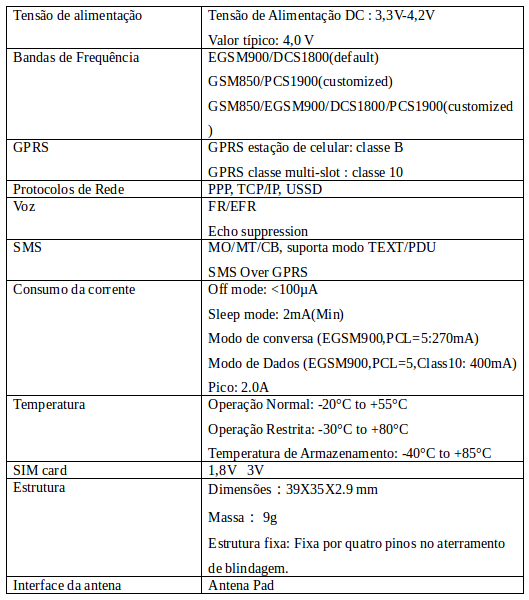
\includegraphics[scale = 0.6]{editaveis/figuras/modulo_spec}
  \label{modulo_spec}
  \caption[Especificações do módulo]{Especificações do módulo. Fonte: \cite{sendtrue08}.}
\end{figure}

Na figura abaixo se encontra o caminho de dados até a central de monitoramento, conhecida como Casa de Máquinas.

\begin{figure}[!h]
  \centering
  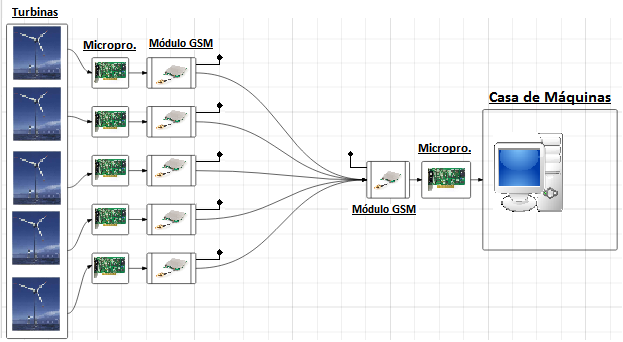
\includegraphics[scale = 0.9]{editaveis/figuras/esquema_transmissao}
  \label{caminho_dados}
  \caption[Caminho de dados]{Caminho de dados.}
\end{figure}

Nas turbinas se encontram sensores que captam informações a cerca do estado de cada turbina, como nível dos reservatórios, rotação das turbinas, vibração da estrutura, etc. Essas informações passam por um processo de tratamento para que se possa transformá-las em sinal digital (isso para sensores que não possuem conversor AC/DC) e posteriormente seus envios. As informações então são passadas para o módulo GSM através dos microcontroladores e depois são transportadas para um mesmo módulo presente na casa de máquinas. Essa transmissão de um módulo para outro pode ser passada como uma mensagem de texto. Escolhe-se esse tipo de transporte, pois se pode enviar protocolos a cerca de cada turbina, ou seja, um pacote de mensagens que são criptografadas nas saídas dos módulos das turbinas até o módulo presente na casa de máquinas. Lá essa mensagem é entendida e passada para o computador e modificada de modo que o usuário possa entender o que cada pacote significa. Esse mesmo processo é feito nos reservatórios onde se encontram as válvulas. Essas válvulas são controladas através de comandos enviados para o microcontrolador, com base nos níveis de água aferidos pelos sensores de níveis nos tanques, abrindo e fechando as válvulas para controlar a vazão da água. 